%%%%%%%%%%%%%%%%%%%%%%%%%%%%%%%%%%%%
% This is the template for submission to MICRO 2021
% The cls file is modified from 'sig-alternate.cls'
%%%%%%%%%%%%%%%%%%%%%%%%%%%%%%%%%%%%

\documentclass[conference]{IEEEtran}


\usepackage{algorithm}
%\usepackage{algorithm2e} %NOT USE IN IEEE Trans
\usepackage{algorithmic}
\usepackage{amsfonts}
\usepackage{amsmath}
\usepackage{amssymb}
%\usepackage{amsthm}
\usepackage{array}
\usepackage{booktabs}
%\usepackage{caption}[font=normalsize]
\usepackage{comment}
\usepackage{enumerate}
\usepackage{enumitem}
\usepackage{float}
\usepackage{graphics}
\usepackage{graphicx} 
\usepackage{lineno}
\usepackage{multirow}
\usepackage{mathtools}
\usepackage{threeparttable}
\usepackage{soul}
\usepackage{url}

% Always include hyperref last
\usepackage[bookmarks=true,breaklinks=true,letterpaper=true,colorlinks,linkcolor=black,citecolor=blue,urlcolor=black]{hyperref}


%%%%%%%%%%%%%%%%%%%%%%%%%%%%%%%%%%%%

\usepackage{textcomp}
\usepackage{xcolor}


\begin{document}

%%%%%%%%%%%---SETME-----%%%%%%%%%%%%%
\title{FeatureBox: Feature Engineering on GPUs\\ for Massive-Scale Ads Systems} 
%%%%%%%%%%%%%%%%%%%%%%%%%%%%%%%%%%%%

\author{\IEEEauthorblockN{Weijie Zhao, Xuewu Jiao, Xinsheng Luo, Jingxue Li, ???, Ping Li}
\IEEEauthorblockA{Baidu Inc.\\
\{weijiezhao, jiaoxuewu, luoxinsheng, lijingxue01, ???, liping11\}@baidu.com}
}

\maketitle
 

%%%%%% -- PAPER CONTENT STARTS-- %%%%%%%%

\begin{abstract}
~~~~\\
~~~~\\
~~~~\\
~~~~\\
~~~~\\
~~~~\\
~~~~\\
~~~~\\
~~~~\\
~~~~\\
~~~~\\
~~~~\\
~~~~\\
~~~~\\
~~~~\\
~~~~\\
\end{abstract}

\begin{IEEEkeywords}
CTR Prediction; GPU; Large-Scale Machine Learning Framework
\end{IEEEkeywords}



\section{Introduction}\label{sec:intro}

Deep learning has been widely employed in many real-world applications, e.g., computer vision~\cite{???}, data mining~\cite{???}, and recommendation systems~\cite{???}. 

In recent years, sponsored online advertising also adopts deep learning techniques to predict the Click-Through Rate (CTR) and make recommendation. Unlike common machine learning applications, the accuracy of the CTR prediction is critical to the revenue. In the context of multi-billion-dollar online ads industry, even a $0.1\%$ accuracy increase will result a noticeable revenue gain. 
We identify two major directions to improve the model accuracy. The first direction is to propose different (or more complicated) model architectures. Every improvement in this direction is considered a fundamental milestone in the deep learning community---this does not happen frequently in the CTR prediction industry.
The other (more practical) direction is feature engineering: to propose and extract new features from the raw training data. The benefit of feature engineering is usually neglected in common deep learning applications because people believe that deep neural networks ``automatically'' extract the features by hidden layers. However, recall that CTR prediction applications are accuracy-critical---the gain of feature engineering is still attractive for in-production CTR prediction models. 
Therefore, in order to achieve a better prediction performance, CTR deep learning models in real-world ads industry tend to utilize larger models and more features extracted from the raw data logs. 

Testing on the historical and online data is the rule-of-the-thumb way to determine whether a new feature is beneficial. Every new feature with positive accuracy improvement (e.g. $0.1\%$) is included into the CTR model. Machine learning researchers and practitioners keep this feature engineering trial-and-error on top of the current in-production CTR model. As a result, the in-production CTR model becomes larger and larger with more and more features. To support the trial-and-error research for new features, it requires us to efficiently train massive-scale models with massive-scale raw training data in a timely manner. Previous studies~\cite{???} propose hierarchical parameter server that trains the out-of-memory model with GPU servers to accelerate the training with GPUs and SSDs. With a small number of GPU servers, e.g., 4, can obtain the same training efficiency as a CPU-only cluster with hundreds of nodes. The training framework focuses on the training stage and assumes the training data are well-prepared---the training data are accessed from a distributed file system.

However, preparing the training data is not trivial for industrial level CTR prediction models---with $\sim 10^{11}$ features. The feature extraction from raw data logs can take a significant proportion of the training time. In addition to the frequent retraining for new feature engineering trials, online ads systems have to digest a humongous amount of newly incoming data to keep the model up-to-date with the optimal performance. For the rapid training demands, optimizing the feature extraction stage becomes one of the most desirable goals of online ads systems.

%the cost of feature extraction is usually neglected in the deep learning community: researchers and practitioners assumes that the training data are cleaned and stored in the disk/memory without further changes. However, online ads systems have to digest newly incoming data to keep the model up-to-date periodically (e.g., daily). 

%Real-world machine learning applications are required to digest a humongous amount of data to obtain the optimal performance. Note that before the actual training, preparing the training data is non-trivial: feature extraction from raw data can take a significant proportion of the training time.


\begin{figure}[htbp]
%\hspace*{-.6cm}
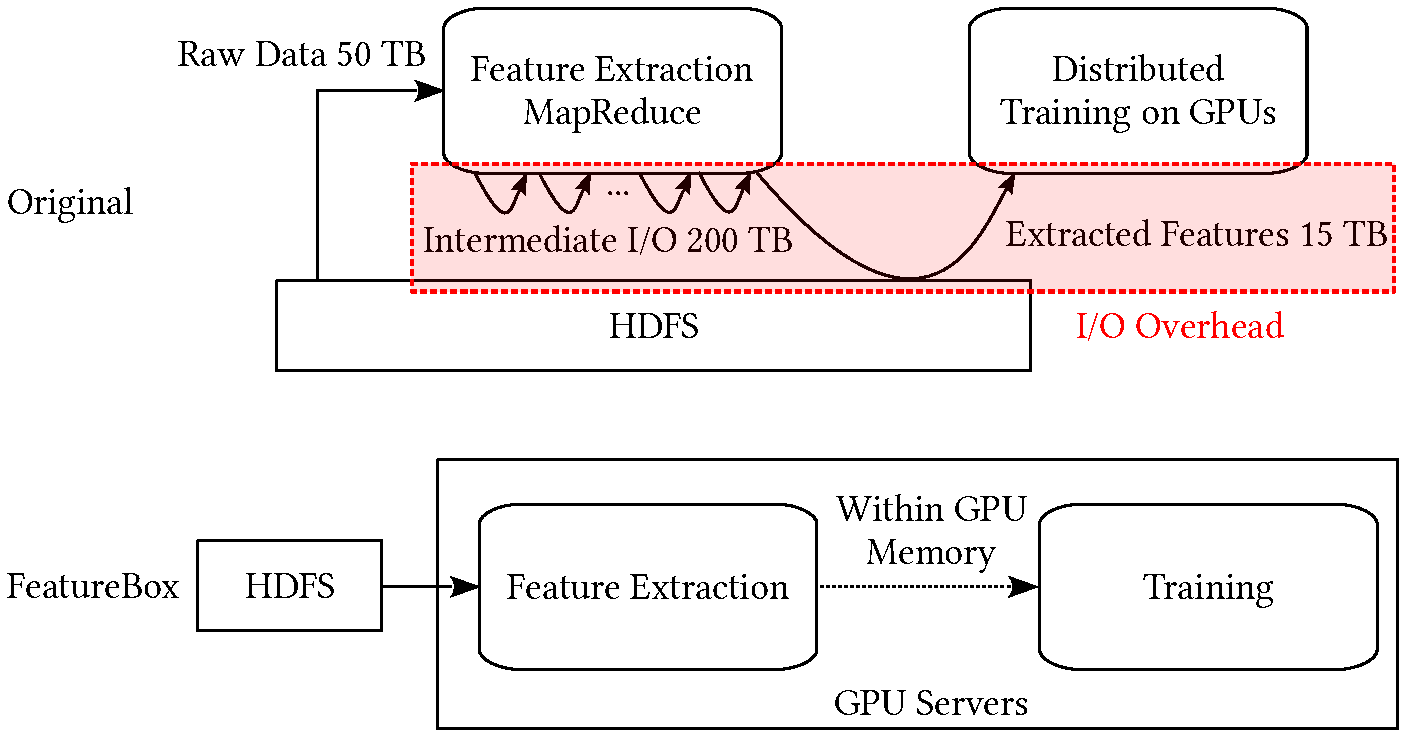
\includegraphics[width=.5\textwidth]{figs/feabox.pdf}
\caption{A visual illustration for the original feature extraction and training workflow (upper); and our proposed FeatureBox (lower).}\label{fig:feabox}
\end{figure}

\textbf{Training workflow.} 
The upper part of Figure~\ref{fig:feabox} depicts a visual illustration of the feature extraction. Due to the large amount of raw data, the original feature extraction task is constructed as MapReduce~\cite{???} jobs that compute feature combinations, extract keywords with language models, etc. Those MapReduce jobs frequently read and write intermediate files with the distributed file system (i.e., HDFS). The intermediate I/O can be as large as 200 TB. After the features are extracted, we also need to materialize them to the $\sim 15$ TB extracted features to the HDFS so that the following distributed training framework can read them from the distributed file system. 
This training workflow incurs rapid communication with HDFS that generates heavy I/O overhead. 

One straightforward question can be raised: \textit{Can we perform the feature extraction within GPU servers to eliminate the communication overhead?} 
In the lower part of Figure~\ref{fig:feabox}, we depict an example for the proposed training framework that combines the feature extraction and the training computation within GPU servers. The intermediate I/O are eliminated by pipelining the feature extraction and the training computation: for each batch of extracted features, we feed the batch to the model training without writing them as intermediate files into HDFS.

\textbf{Challenges}
However, moving the feature extraction to GPU servers is non-trivial. Note that the number of GPU nodes is much fewer compared with the CPU-only cluster. We recognize three main challenges in putting the feature extraction into GPU servers:
\begin{enumerate}
\item Network I/O bandwidth. The network I/O bandwidth of GPU servers is orders of magnitude smaller than the bandwidth of CPU clusters because we have fewer nodes---the total number of network adapters is fewer.   
\item Computing Resources. With the fewer number of nodes, the CPU computing capability on GPU servers is also orders of magnitudes less powerful than the CPU cluster. We have to move the original CPU computations to GPU operations.
\item Memory Usage. The feature extraction process contains many memory-intensive operations, such as dictionary table lookup, sort, reduce and so on. We have to design an efficient memory management system to perform these memory-intensive operations on GPU servers with limited memory.
\end{enumerate}

\textbf{Contributions.} 
We summarize our contributions of this paper as follows:
\begin{itemize}
\item We propose FeatureBox, a novel training framework that combines the feature extraction and training in the same pipeline. 
\item We present a column-store that incrementally reads the data logs??? to reduce network I/O.
\item We materialize frequently-used features as a view so that we can reuse this view without extra computations.
\item We introduce a main memory and GPU memory management algorithm that adaptively schedules computing operators.
\item The experimental results on real-world ads applications confirm the effectiveness of our proposed methods.
\end{itemize}

\section{Preliminary}
In this section, we present a brief introduction of CTR prediction models and the distributed GPU parameter server. Both concepts are the foundations of our proposed FeatureBox. 

\subsection{CTR Prediction Models}

\subsection{Distributed GPU Parameter Server}

\section{FeatureBox Overview}



\section{Related Work}

\section{Conclusions}


\bibliographystyle{IEEEtran}
%\bibliography{biblio}
%%%%%%%%%%%%%%%%%%%%%%%%%%%%%%%%%%%%

\end{document}